\documentclass[12pt]{article}
\usepackage[margin=1in]{geometry}
\usepackage{float}
\usepackage{enumitem}
\usepackage{indentfirst}
\usepackage{graphicx}

\setlength{\parindent}{0pt}

\title{Placing a Diner in Brooklyn, NY\thanks{To your mother}}
\author{	Joseph Mifsud  \\
		Hungry for Opportunity}
\date{\today}

\begin{document}
\maketitle
\begin{abstract}

	A study was performed to identify optimal locations to open a diner catering to the hipster demographic in Brooklyn, NY. 
	Brooklyn was algorithmically tessellated into a hexagonal grid of neighborhoods. 
	Foursquare's Places API was used to fetch data on a set of relevant venues in each neighborhood. 
	Neighborhoods were clustered with DBSCAN to identify neighborhoods of low hipster-density. 
	A cost-function was defined to optimize the ratio between the target demographic and competitive venues.
	Four locations of were identified to a position within 600m.
\end{abstract}

\section{Introduction}
\subsection{Background}
	The cozy and relaxed nature of a diner makes them a popular option for dining out.
	As a small business, the diner offers its stakeholders the opportunity for lucrative financial gain within a relatively short amount of time.
	A well-placed diner has greater opportunity for success than the misplaced.
	Siting a diner in Brooklyn requires defining a target market.
	
	Brooklyn NY's estimated population of 2.6 million yields one of the most diverse and competitive markets for the food service industry in the world.
	Of Brooklyn's most affluent denizens are the members of the contemporary hipster subculture.
	According to Wikipedia, the term hipster is "mostly associated with perceived upper-middle-class white young adults who gentrify urban areas."
	The contemporary hipster is a subset of the Millenial generation which makes up 27\% of the population and contributes \$1.3 trillion in annual consumer spending.
	Hipsters have considerable purchasing power.
	Therefore, it is advantageous for entrepreneurs tapping into this market to accurately determine locations conducive to their venture.
	
\subsection{Problem}	
	Locating the target demographic as well as competitive regions requires an assumption and data.
	The assumption made is that regions with organic grocery stores, independent movie theaters, bicycle shops, and flea markets indicate the presence of members of the target demographic.
	This assumption is entirely heuristic.
	Notwithstanding, precedence for this technique is provided by MoveHub, a British marketing and logistics firm, who created a "Hipster Index" in 2017 using similar types of venue.

	The data required is the the location and type of venues, both hipster and competitive, in Brooklyn.
	This project aims to find locations where the target demographic is and competition is not.
	Further, an attempt is made to prefer locations that are located near major transportation infrastructure such as the Brooklyn, Manhattan, and Williamsburg Bridges.

\subsection{Interest}
	This information is most valuable to entrepreneurs. 
	In addition, the information extracted from this study may also be of interest to real estate developers and investors.
	Other interested parties may include those conducting research on demographics in the region.

\section{Data} \label{documentclasses}
\subsection{Data Sources}
	There were three types of data collected for this study.
	First, coordinates from OSM's Geocoding API were used to define a target region for the study.
	Second, addresses from OSM's Reverse Geocoding API were used to associate an address with each subregion, or neighborhood, within the target region.
	Finally, Foursquare's Places API provided the venue data necessary for this study.
	
	The venue data is the largest component of the project on a storage size basis.
	For each neighborhood, it contains information for each venue.
	The data provided by Foursquare for venues include a unique ID, the name, its geographic coordinates, a category indicating type, as well as the distance between the queried point and the venue in meters.
	For example the category might be "Tire Shop" or "Fast Food Restaurant."
	This category data is used to identify competition for the proposed diner such as cafes.
	In addition, venue categories were used as an indicator for neighborhoods that contain the target demographic.

\subsection{Data Cleaning}
	There were two aspects of the data that were considered for cleaning.
	First, the target region included areas of the Hudson River Estuary.
	Obviously, neighborhoods in Upper New York Bay are not be suitable for recommendation to stakeholders.
	These neighborhoods were not removed from the study or treated any differently that any other neighborhood.
	It was correctly believed that analysis would not lead to a recommendation of these areas in the first place.

	The second aspect of the data concerns the categorical values from the Places API.
	It is the case that a single venue may belong to multiple categories.
	For example, Whole Foods Market may belong to the "Organic Grocery Store" category and the "Grocery Store" category.
	For this reason, when a request was sent for organic grocery stores the venues returned may or may not include the category "Organic Grocery Store."
	To remedy the case of secondary categories, a list was compiled of all the categories returned by Foursquares Places API when queried with the venues defined as indicators for the presence of the target population.
	If a venue's category was on this list, it would be considered an indicator of the presence of members of the hipster subculture.

\subsection{Feature Selection}
	This study is primarily concerned with three characteristics of a neighborhood.
	\begin{enumerate}[noitemsep]
		\item Whether or not if contains members of the hipster subculture
		\item The amount of competition
		\item The location in relation to major transportation infrastructure 
	\end{enumerate}
	
	Features were selected to capture information related to these characteristics.
	In an effort to indicate the presence of members of the hipster subculture, specific categories of venues were queried.
	These venues are the following: 
	\begin{center}	
	\begin{tabular}{ c c }
		Organic Grocery Store & Bike Shop \\
		Indie Movie Theater & Flea Market \\
	\end{tabular} \\
	\end{center}
	It is noted that no restaurants or coffee shops are used to indicate the presence of the target market.
	Restaurants and coffee shops will be competing with the proposed diner. 
	They are sought when selecting features identifying the characteristics of the competition.	
	The categories of venue used to locate and quantify the competition were: 
	\begin{center}
	\begin{tabular}{c c c c}
		Diners & Coffee Shops & Cafes & Breakfast Spots \\
		Burger Joints & Sandwich Places &Greek Restaurants \\
	\end{tabular}
	\end{center}
	
	It is self-evident that the location of a neighborhood will be critical in determining where to place the proposed establishment.
	All locations in the study are communicated in latitude and longitude until the final results are given.
	In the results section, the coordinates of locations are translated to a street address.

\section{Methodology}
\subsection{Exploratory Data Analysis}

\begin{figure}[h!]
	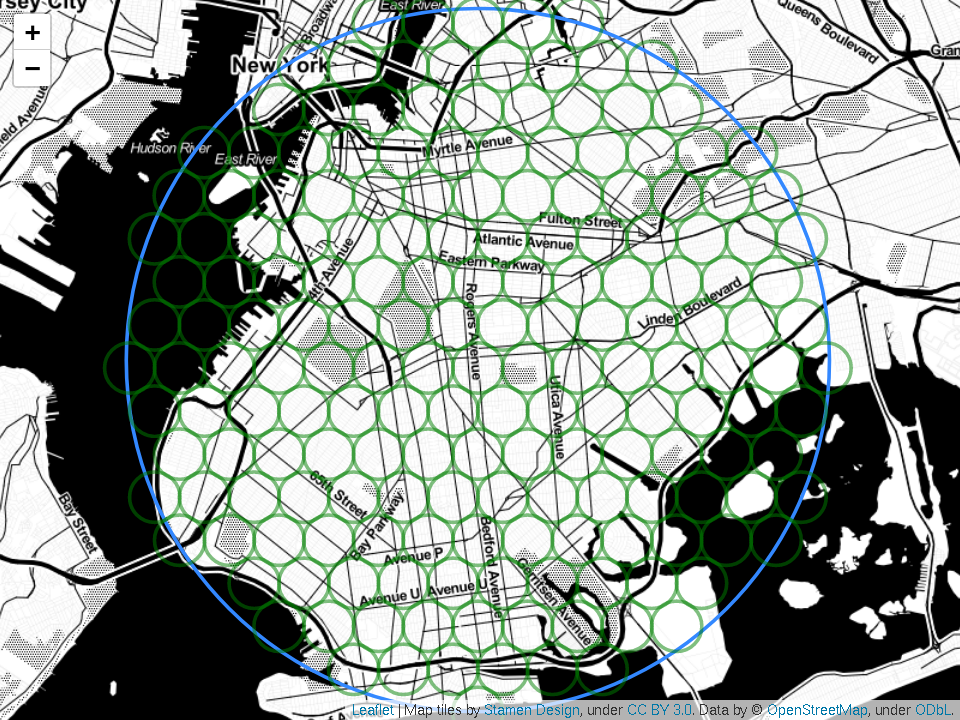
\includegraphics[width=6.5in]{citymap.png}
  \caption{A map of the studied neighborhoods.}
  \label{fig:citymap}
\end{figure}
	The target region of Brooklyn has been divided into 183 circular areas with a radius of 600m.
	Each circular area, referred to as a neighborhood, has been assigned a neighborhood number to uniquely identify it.
	Figure \ref{fig:citymap} is a map of the target region which shows the boundaries of each neighborhood in this study.
	Venues, both indicative of hipsters and the competition, were fetched from Foursquare for each neighborhood.
	In total, data from 3024 venues were collected.

\begin{figure}[H]
  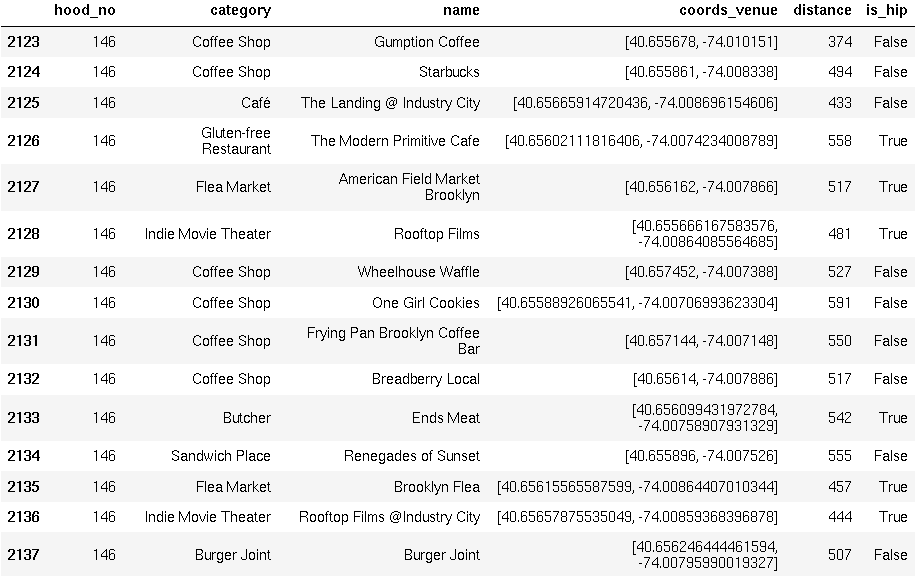
\includegraphics[width=6.5in]{hood146.png}
  \caption{A sample of typical neighborhood data}
  \label{fig:hood146}
\end{figure}

	Figure \ref{fig:hood146} is a sample of the data for neighborhood number 146.
	There are multiple columns in \ref{fig:hood146}
	The "hood\_no" column indicates to which circular neighborhood, described in figure \ref{fig:citymap}, the venue belongs.
	There is a column to hold the primary category which described the venue.
	As mentioned above, it is possible that a venue belong to more than one category.
	The "name" column is self-explanatory.
	The "coords\_venue" parameter holds onto the geographic coordinates for each venue measured in degrees North and West.
	"Distance" describes the displacement of the venue from the neighborhood of corresponding neighborhood number.
	Finally, there is a column to keep track of whether the venue is considered relevant to the target market or to the competition.
	All venues were plotted onto a map of Brooklyn in figure \ref{fig:venues_map}.
profile 
\begin{figure}[H]
  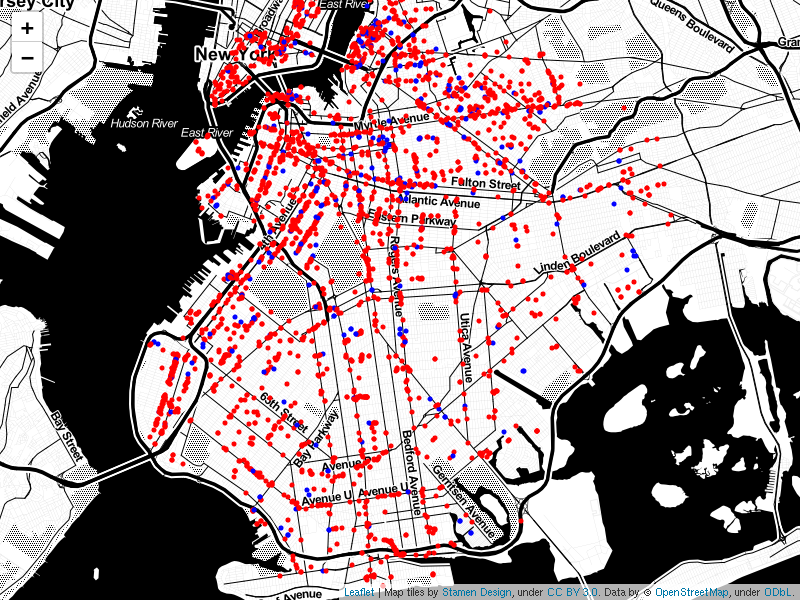
\includegraphics[width=6.5in]{venues_map.png}
  \caption{A map of the target region. Venues that are in competition with a proposed diner are plotted in red. Venues indicating the presence of hipsters are in blue.}
  \label{fig:venues_map}
\end{figure}

	The map of venues suggests that there are more venues closer to Manhattan than Jamaica Bay.
	To get a better understanding of what is going on, a heat map of the venues indicating the target market was created.
\begin{figure}[H]
  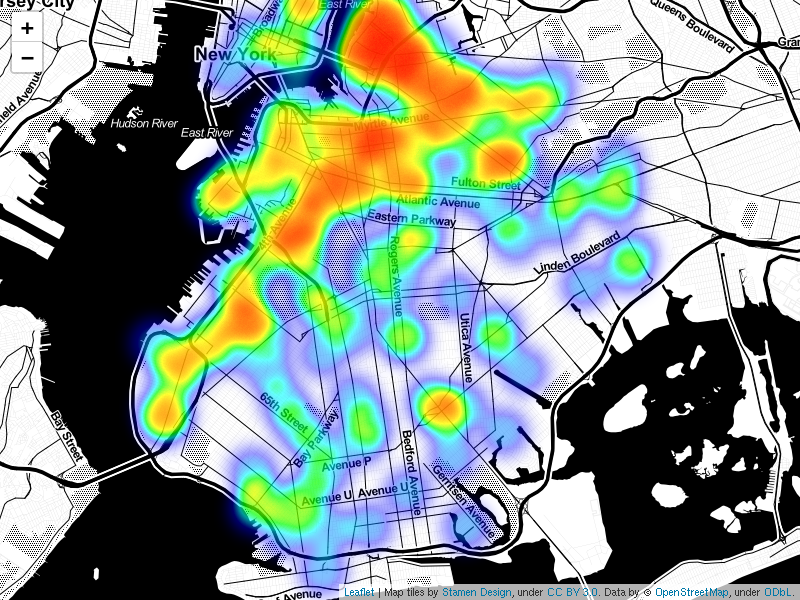
\includegraphics[width=6.5in]{hipster_heatmap.png}
  \caption{A heat map of venues which indicates the presence of members of the hipster subculture.}
  \label{fig:hipster_heatmap}
\end{figure}
	Figure \ref{fig:hipster_heatmap} shows the density of hipster venues in the target region.
	The density of hipster-venues varies throughout Brooklyn.
	This suggests that some areas will be more well-suited for a diner catered to this demographic.
	There is the greatest density of hipster venues in the regions between the East River and Jamaica Avenue as well as the Upper New York Bay and the Fort Hamilton Parkway.
	In the analysis portion of this study an attempt will be made to cluster neighborhoods together on the density of hipster venues.
	The goal of such a clustering will be to separate neighborhoods that have a low hipster density.
	It is likely that in the end of our study, a neighborhood indicated by this heat map will be recommended as suitable for the proposed diner.
	
	Correspondingly, a heat map was created to visualize the competition in the region.
\begin{figure}[H]
  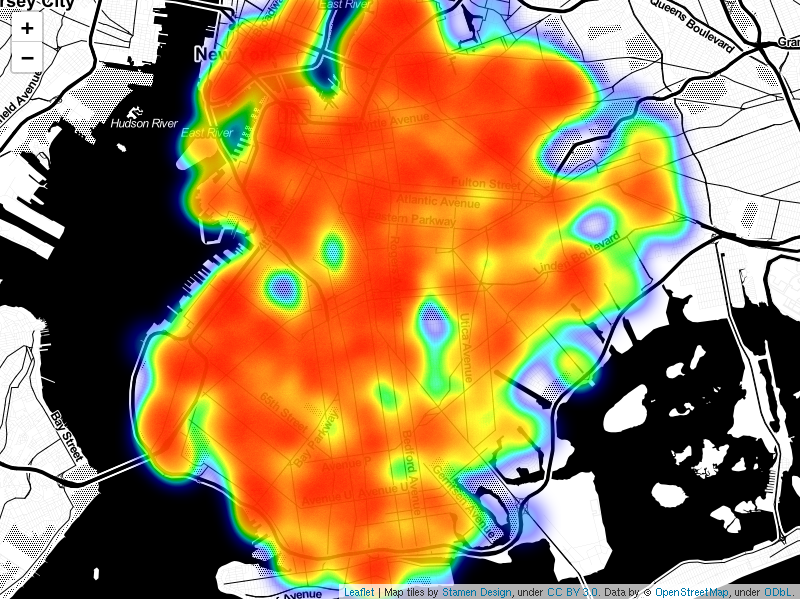
\includegraphics[width=6.5in]{comp_heatmap.png}
  \caption{A heat map of venues in direct competition with the proposed diner.}
  \label{fig:comp_heatmap}
\end{figure}
	Figure \ref{fig:comp_heatmap} shows the density of venues in competition with the proposed diner.
	The competition heat map suggests that competition is relatively consistent throughout Brooklyn.
	There may be slightly more competition in the regions found to have the greatest density of hipster-venues.
	A hypothesis test could determine whether or not these regions deviate enough from the mean to be considered significantly different from the overall population of neighborhoods.
	If the author had mor time, a hypothesis test would be conducted to confirm what the heat map is suggesting.
	It is now assumed that the profile of regions varies with respect to the amount of hipster venues.
	Each neighborhood holds a unique location in venue space.

	To locate a neighborhood in venue space, a vector composed of the quantity of each type of category is used.
	Hipster-space is a subset of venue-space and includes only the categories defined as indicators of the presence of members of the hipster subculture.
	An array was created to hold the quantity of each type of hipster venues for each neighborhood.
	Each neighborhood had the z-score computed for each type of hipster category.
	The greater the z-score for each of the hipster categories within a neighborhood, the more likely that there is a presence fo hipsters in the neighborhood.
	Below is a sample of the array containing the vectors for four neighborhoods.\\
\begin{center}
\begin{tabular}{r c c c c }

Neighborhood	&Bike Shop & Flea Market  &Indie Movie Theater  &Organic Grocery\\
	143		 &0	       &0                    &0                &0\\
	144              &1            &0                    &1                &0\\
	145              &1            &2                    &0                &0\\
	146              &0            &2                    &2                &0\\
\end{tabular}
\end{center}

	Histograms were created to visualize the z-score frequency of the hipster-indicating venues. 	\\
\begin{figure}[H]
  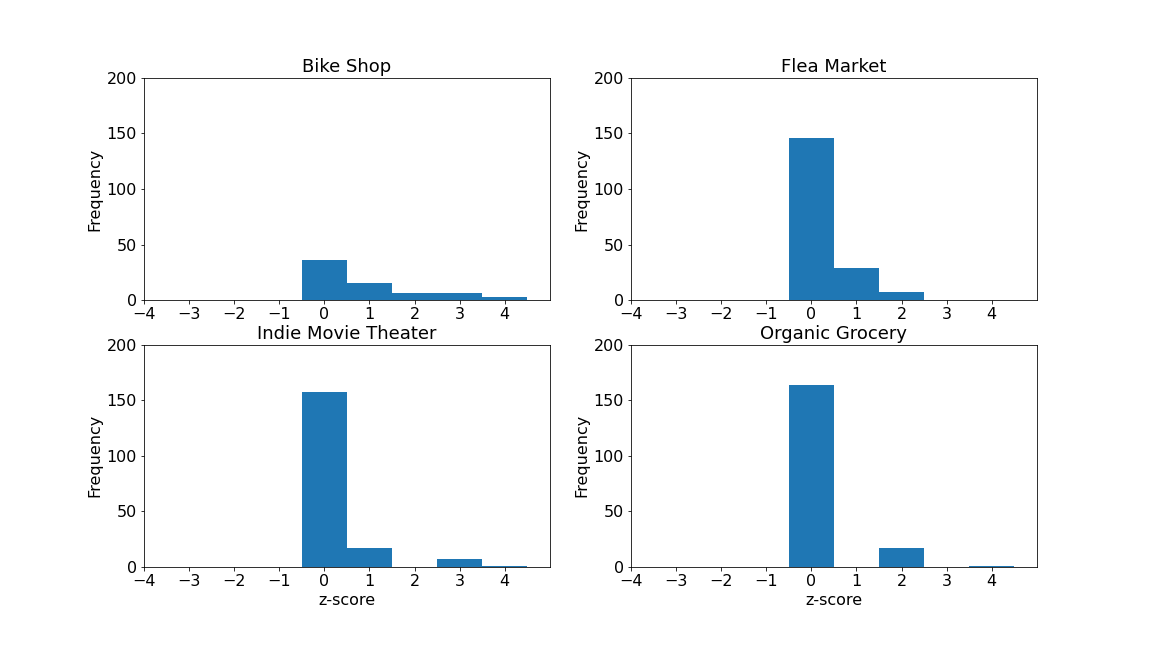
\includegraphics[width=6.5in]{zscores.png}
  \caption{Z-scores were calculated for venues that indicate the presence of hipsters}
  \label{fig:zscores}
\end{figure}
	The z-score histograms for the hipster-venues are all significantly skewed to the right. 
	Obviously, this indicates the lower bound for the number of venues a neighborhood can have.
	It is likely that the z-score distribution for all types of venue skew to the right since they all share this feature.
	Below descriptive statistics for the selected categories are tabulated.\\
\begin{center}
\begin{tabular}{c c c c c}
			& Bike Shop 	& Flea Market 	& Indie Movie Theater	& Organic Grocery	\\
	$\bar{x}$	& 0.699		& 0.279		& 0.213			& 0.126		\\	
	$\sigma$	& 1.246		& 0.766		& 0.623			& 0.433		\\
	Median		& 0		& 0		& 0			& 0		\\
	Mode		& 0 (117)	& 0 (146)	& 0 (157)		& 0 (164) 	\\
	Skew		& 2.327		& 6.175		& 4.052			& 5.146 	\\
\end{tabular}
\end{center}
\subsection{Machine Learning}
	An attempt was made to cluster neighborhoods according to the density of hipster-indicative venues.
	The strategy was to cluster together neighborhoods of low-density.
	Those that remain after clustering have any density except low-density.
	To select a value for epsilon in DBSCAN, the k-nearest neighbor algorithm was used to find the distance between points.
\begin{figure}[H]
  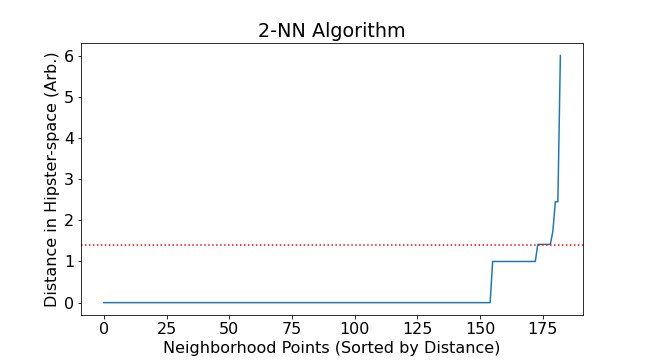
\includegraphics[width=6.5in]{knn.png}
  \caption{The distance between points was calculated with kNN.}
  \label{fig:knn}
\end{figure}
	The graph shows that about 80\% of the neighborhoods are within a distance of one from the origin of hipster-space.
	By setting $\epsilon$ in DBSCAN equal to 1.4, DBSCAN will group together the neighborhoods that have hipster venues within 1.4 distance units from a core point.
	Neighborhoods will be considered core points if they have a minimum number of points within a distance $\epsilon$ of the it.
	Using the good-choice method, the minimum number of points required to be considered a cluster was set to 9.
	This will have the effect of not creating multiple small clusters around irregular features in the data.
	These irregular neighborhoods will be assigned to the outlier cluster.

	DBSCAN created four clusters from the data.
	The number of neighborhoods in each cluster is given as follows:
\begin{itemize}[noitemsep]
	\item Cluster 0:	138
	\item Cluster 1:	9
	\item Cluster 2:	11
	\item Outliers:		25
\end{itemize}

	A map of the clusters generated is visualized in figure \ref{fig:cluster}.
	Each neighborhood is represented on the map by a circle of radius 600m.
	The color of the circle represents the cluster membership for that neighborhood.
	Each color was generated algorithmically to give maximum distinction between colors.
	For a number of clusters less than seven, this strategy gives visually distinct results.
	For a large number of clusters, a different visualization strategy must be employed.
\begin{figure}[H]
  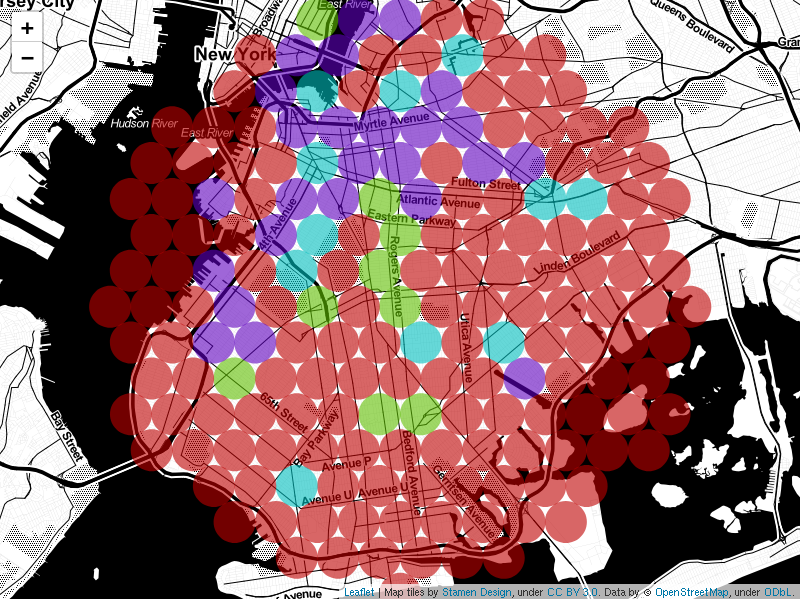
\includegraphics[width=6.5in]{cluster.png}
  \caption{The distance between points was calculated with kNN.}
  \label{fig:cluster}
\end{figure}
\subsection{Optimization}
	To select one neighborhood over another for the proposed diner, a cost-function was defined.
	The cost function was defined to account for for the criteria set forth in the business problem.
	In summary, these criteria are that a location must have:
\begin{enumerate}[noitemsep]
	\item Many hipsters, as close as possible
	\item Little competition, as far away asd possible.
	\item A short distance between the neighborhood and major transportation infrastructure.
\end{enumerate}
	To describe if a venue is close by, a function was defined to calculate the venue's closeness.
	The data provided by Foursquare is how far away a venue is from a neighborhood.
	This is related to how close it is, but also the opposite.
	Therefore it was said that the closeness $C$ of a venue is given by the equation:\\

$\displaystyle{C(d_v) = \frac{D_{max} - d}{D_{max}}}$ \\

Where:
\begin{itemize}[noitemsep]
	\item	$D_{max} - maximum\ distance\ to\ any\ venue$
	\item	$d_v - distance\ to\ venue\ v$
	\item	$C(d_v) -\ Closeness\ of\ venue\ v$
\end{itemize}
		
	It was necessary to calculate the closeness of both hipster venues as well as competitive ones.
	To mirror this fact, venue space was subdivided into hipster-space and competition-space.
	Hipster-space contains the coordinates, in number of hipster-type categories, for all neighborhoods.
	Competition space is then defined similarly for all types of category that are not those designated to be indicative of hipsters.
	A proximity score $X_H$ was then calculated to reflect the number and proximity of both hipster venues and competitive venues for each neighborhood.\\

$\displaystyle{\vec{X_{H}} = \sum_{h}(C\left(d_{h}\right) + 1)\hat{h} + \sum_{c}(C\left(d_{c}\right) + 1)\hat{c}}$\\

Where:
\begin{itemize}[noitemsep]
	\item $X_{H}(d)-\ proximity\ score\ of\ neighborhood\ H$
	\item $d_h -\ distance\ to\ hipster\ venue$
	\item $d_c -\ distance\ to\ competition\ venue$
	\item $\hat{h} -\ hipster\ space$
	\item $\hat{c} -\ competition\ space$
\end{itemize}

	The Haversine equation was used to calculate the distance for each neighborhood and each of the three bridges.
	The Haversine equation, given two pair of coordinates in degrees North and West, calculates the great-circle distance between the two points.
	Of the three distances for each neighborhood, the smallest one is included as a ratio to the diameter of the target region in the scoring vector $\vec{S}$ as component $\vec{B_H}.$\\

	The Haversine Equation:\\

$\displaystyle{H(\phi,\lambda) = 2r\arcsin\left(\sqrt{\sin^2\left(\frac{\phi_2 - \phi_1}{2}\right) + \cos(\phi_1) \cos(\phi_2)\sin^2\left(\frac{\lambda_2 - \lambda_1}{2}\right)}\right)}$\\


$\displaystyle{ \vec{B_H} = min(\frac{H(\rho_{H},\rho_{b})}{2r_{bk}})\hat{b} }$\\
	
	The bridge component is added to the proximity score to create the score vector.\\

$\displaystyle{\vec{S_H} = \vec{X_H} + \vec{B_H}}$

$\displaystyle{\vec{S_H} = h\hat{h} + c\hat{c} +b\hat{b}}$\\

	An array of containing the components of the score vector for each neighborhood was created.
	Each component of the score vector describes one of the criteria set forth for the business problem.
	A sample of the score vector values for is shown below.
\begin{center}
\begin{tabular}{ c c c }
	$\hat{h}$	&$\hat{c}$	&$\hat{b}$ \\
		0.          &2.76836158  &0.85471729 \\
		0.         &12.1819209   &0.73645233 \\
		1.40451977 &19.66892655  &0.75877421 \\
		4.16271186  &3.03615819  &0.78680609 \\
		0.          &1.8779661   &0.81996254 \\
\end{tabular}
\end{center}
	
	A cost function was then defined to value each neighborhood's score vector.
	The objective of the cost function is to rank neighborhood in their ability to satisfy the criteria of the business problem.
	It was arbitrarily chosen that the lowest values produced by the cost function would be the neighborhoods that best meet the criteria.
	The cost function was defined as follows:
\begin{center}
$\displaystyle{O_H = -h +h\frac{c}{C_{max}}+(1+b)^2}$
\end{center}	

	There are three terms in the cost function.
	The first term is the negated hipster component of the score vector.
	Neighborhoods with a large hipster component are preferred in this way.
	The term is negated because of the decision to make the objective of the best neighborhood as small as possible.
	The second term of the cost function is the product of the hipster component of a neighborhood with the ratio of the neighborhoods competition component and the maximum competition component of any neighborhood.
	This term will penalize neighborhoods that have a large hipster component as well as a large competition component.
	Finally, the third term is related to the square of the bridge component.
	This term is added to select from multiple neighborhoods with similar competition and hipster scores the one closest to the bridges.

	The value of the cost function was calculated for each neighborhood.
	A hexadecimal color value was generated for each neighborhood based upon its cost-function value.
	A list was created of the neighborhoods with the lowest cost function values.
	The results were plotted onto the map in figure \ref{fig:scoremap}.\\
\begin{figure}[H]
  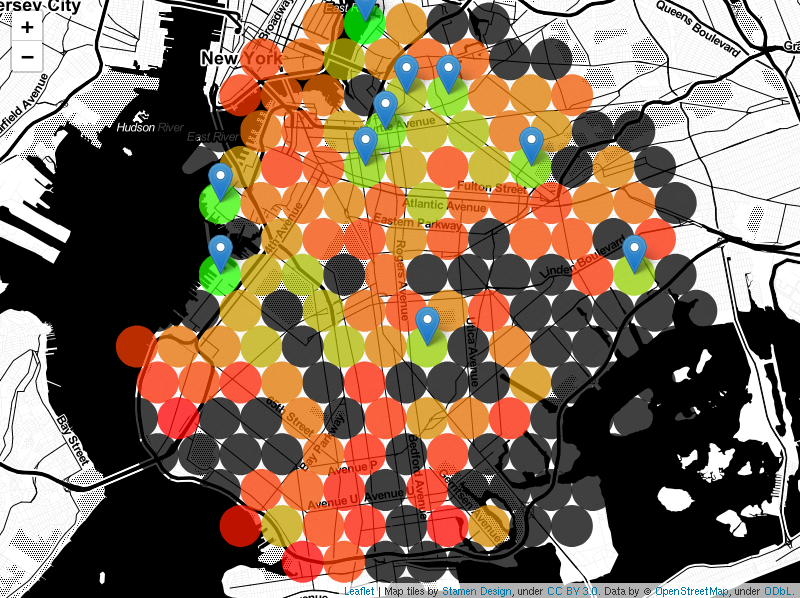
\includegraphics[width=6.5in]{scoremap.png}
	\caption{The cost function was evaluated for each neighborhood. Neighborhoods with the lowest score are marked.}
  \label{fig:scoremap}
\end{figure}

\section{Results}

	A list of  ten neighborhoods with the lowest cost-function values was compiled.
	An inner join was performed with all clusters with the exception of cluster number 0.
	Including regions of open water, cluster 0 is a low-hipster density cluster.
	The following list was produced.
	Optimal locations are within 600m of the points specified.
	
\begin{enumerate}[noitemsep]
	\item 748 Chauncey Street, Brooklyn New York 11207
	\item 127 Saint James Place, Clinton Hill Stone Street Historic District 
	\item 221 Middleton Street, Brooklyn New York 11206
	\item 226 Moore Street, Brooklyn New York 11206
	\item North 10th Street Brooklyn, Kings County 11211 
	\item 1377 Brooklyn Avenue, Brooklyn Community District 17, New York
	\item 52 39th Street, Sunset Park Stone Street Historic District 
	\item 371 Van Brunt Street, Red Hook Stone Street Historic District 
	\item 868 Bedford Avenue, Brooklyn New York 11205
\end{enumerate}

	Figure \ref{fig:csmap} marks the neighborhoods above on the DBSCAN cluster map.

\begin{figure}[H]
  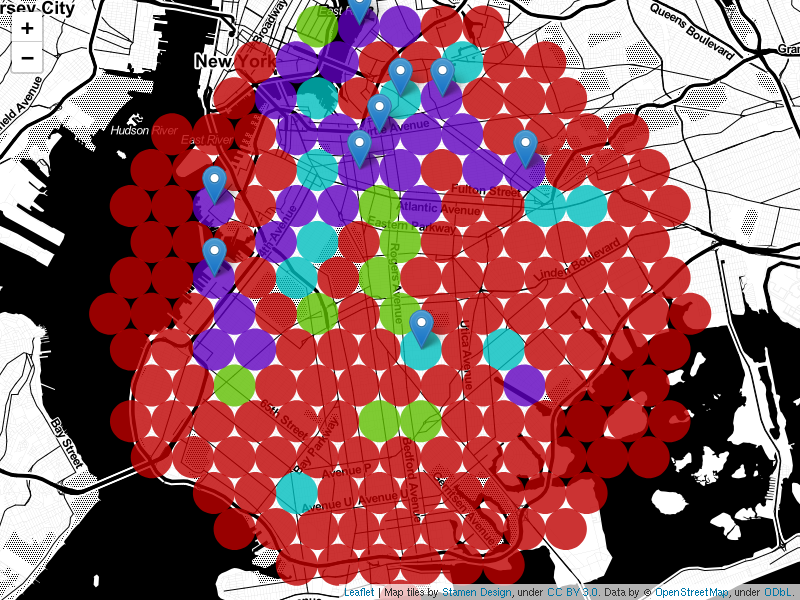
\includegraphics[width=6.5in]{csmap.png}
	\caption{The cost function was evaluated for each neighborhood. Neighborhoods with the lowest score are marked.}
  \label{fig:csmap}
\end{figure}

\section{Discussion}
	Two models were used to analyze this data.
	The first model was produced by using the DBSCAN algorithm to cluster all neighborhoods based upon the quantity of venues deemed to be hipster related within.
	This model produced four clusters.
	DBSCAN created a cluster that includes regions of Upper New York Bay and many neighborhoods in the target region.
	This is remarkably revealing.
	Neighborhoods in this cluster have low-hipster venue density.

	The second model used was a purpose designed cost function.
	The cost function model valued each neighborhood according to the criteria set for by the business problem.
	Neighborhoods selected by this model are in different regions of Brooklyn.
	Remarkably, there is a correlation between the two models.
	Nine of ten neighborhoods with the lowest cost function value also clustered out of of the low-density cluster.

	There is agreement between the models.
	Both models indicate the neighborhoods specified meet the criteria of the business problem.
	The locations specified are recommended for further review by stakeholders.

\section{Conclusion}\label{conclusions}
	There are many people who live in New York City's borough of Brooklyn.
	This gives rise to different demographic profiles in different regions.
	These regions can be targeted to market to specific audiences.
	Through data science these profiles and regions may be revealed.
\end{document}
